%
% `author_guide.tex' - AIAA author instructions that use the AIAA class.
%
% Typical processing for PostScript (PS) output:
%
%  latex author_guide
%  bibtex author_guide  (bibliography)
%  makeindex -s nomencl.ist -o author_guide.gls author_guide.glo (nomenclature)
%  latex author_guide   (repeat as needed to resolve references)
%
%  xdvi author_guide    (onscreen draft display)
%  dvips author_guide   (postscript)
%  gv author_guide.ps   (onscreen display)
%  lpr author_guide.ps  (hardcopy)
%
% Note: With the above, only Encapsulated PostScript (EPS) images can be used.
%
% Typical processing for Portable Document Format (PDF) output:
%
%  pdflatex author_guide
%  bibtex author_guide  (bibliography)
%  makeindex -s nomencl.ist -o author_guide.gls author_guide.glo (nomenclature)
%  pdflatex author_guide      (repeat as needed to resolve references)
%
%  acroread author_guide.pdf  (onscreen display)
%
% Note: If you have EPS figures, you will need to use the epstopdf
% script to convert them to a form compatible with PDF.   Depending
% on your version of pdflatex, it accepts a variety of other image
% formats such as JPG, TIF, PNG, and so forth -- check your documentation.
%
% If you do *not* specify suffixes when using the graphicx package's
% \includegraphics command, latex and pdflatex will automatically select
% the appropriate figure format from those available.  This allows you
% to produce PS and PDF output from the same LaTeX source file.
%
% To generate a large format (e.g., 11"x17") PostScript copy for editing
% purposes, use
%
%  dvips -x 1467 -O -0.65in,0.85in -t tabloid author_guide
%
% Copyright (C) 2004 by Bil.Kleb@NASA.Gov, Bill.Wood@NASA.Gov,
% and ErichK@AIAA.org.

\documentclass{aiaa-tc}% add 'draft' option to graphically depict overfull boxes

 \usepackage{wrapfig}% embedding figures/tables in text (i.e., Galileo style)
 \usepackage{threeparttable}% tables with footnotes
 \usepackage{dcolumn}% for decimal-aligned tabular math columns
 \usepackage{nomencl}% automatic nomenclature generation via makeindex
 \usepackage{subfigure}[1995/03/06]% subcaptions for subfigures
 \usepackage{subfigmat}% for matrices of similar subfigures, aka small mulitples
 \usepackage{fancyvrb}% for extended verbatim environments
 \usepackage{lettrine}% dropped capital at beginning of paragraph
 \usepackage[dvips]{dropping}% alternative dropped capital package
 \usepackage{hyperref}% embedding hyperlinks [must be loaded after dropping]

 % decimal-aligned tabular column [dcolumn.sty]
 \newcolumntype{d}{D{.}{.}{-1}}

 % collects nomenclature entries [nomencl.sty]
 \makeglossary

 % Verbatim defaults [fancyvrb.sty]
 \fvset{fontsize=\footnotesize,xleftmargin=2em}

 \title{Preparation of Papers for\\
        AIAA Technical Conferences}

 \author{%
  First A. Author\thanks{Job Title, Department, Address, and AIAA
                              Member Grade.}
  \ and
  Second B. Author\thanksibid{1}\\% same footnote as 1st author\\
  {\normalsize\itshape
   Business or Academic Affiliation, City, Province, Zipcode, Country}\\
  \and
  Third C. Author\thanks{Job Title, Department, Address, and AIAA
                              Member Grade.}\\
  {\normalsize\itshape
   Another Business or Academic Affliation, City, Province, Zipcode, Country}
 }

 \AIAApapernumber{200?-????}
 \AIAAconference{Conference Name, Date, and Location}
 \AIAAcopyright{\AIAAcopyrightD{200?}}

 % define some commands to maintain consistency
 \newcommand{\pkg}[1]{\texttt{#1}}
 \newcommand{\cls}[1]{\textsf{#1}}
 \newcommand{\file}[1]{\texttt{#1}}

\begin{document}

\maketitle

\begin{abstract}
These instructions give you guidelines for preparing papers for AIAA
Technical Conferences.
Use this document as a guide if you are using \LaTeXe.
Otherwise, use this document as an instruction set.
Should this submission be for a non-electronic meeting, the electronic
file of your paper will be formatted further at AIAA.
Define all symbols used in the abstract.
Do not cite references in the abstract.
The footnote on the first page should list the Job Title and AIAA Member
Grade for each author.
\end{abstract}

% creates nomenclature section when processed by MakeIndex
\printglossary

\section{Introduction}

\lettrine[nindent=0pt]{T}{his} document is a \LaTeX\ template.
If you are reading a hardcopy or PDF version of this document, please
download the \LaTeX\ macros and sample files from
\href{http://www.ctan.org/}{www.ctan.org}
so you can use it to prepare your manuscript.
The \cls{aiaa-tc} class uses Computer Modern (CM) fonts, which
are part of any standard \TeX installation.
Use the \LaTeX\ files for formatting purposes,
but please see \file{author\_guide.pdf} for specific layout instructions.
Authors will first need to save the \cls{AIAA} files to their
working directory or install them into their \TeX\ distribution.

\section{Procedure for Paper Submission}

All manuscripts are to be submitted electronically via the AIAA
submission tool at \href{http://www.aiaa.org/author}{www.aiaa.org/author}.
Select the ``Submit a Paper to an AIAA Conference'' link, then click the
``Edit Old'' button.
When you submitted your abstract for review, you should have received a
tracking number for your paper.
Use this tracking number, along with the last name of the corresponding
author, to gain access to the AIAA Author Status Page.
This site will allow you to track your paper's status, update submission
data, select a copyright statement, and upload your manuscript.

Before you can upload your manuscript, you will need to select a
copyright statement to appear on your paper.
This can be achieved by clicking the ``Copyright Information'' link on
the Author Status Page.
Be sure to read the instructions and specific statements carefully
before selecting a statement for your manuscript.

Once you have selected a copyright statement, you can use the ``Upload
Manuscript'' feature of the Author Status Page to upload your paper.
All accepted authors will be notified by AIAA of the relevant
submission deadlines.
In addition, the deadlines for every conference can be found under the
conference title on the Author Status Page.

As with the submission of your abstract, be sure the name of the file
you upload for processing is short and simple (i.e., ``msc12345.tex'')
with no spaces, tildes, symbols, or other unusual characters.
If the file being uploaded is in \LaTeX, the document must be based
on \cls{article.cls} (this AIAA class is based on this class).
Failure to meet these requirements could result in a processing error
that would require you to re-upload your manuscript.%
\footnote{If you are uploading a PDF or postscript file, please do not
  include foreign (i.e., non-Roman alphabet) fonts.}
If you encounter difficulties with the upload and/or conversion of your
manuscript, please contact AIAA Papers Tech Support for assistance at
\href{mailto:paper_tech_support@aiaa.org?subject=upload}%
     {paper\_tech\_support@aiaa.org}.

\section{General Guidelines}

The following section outlines general (non-formatting) guidelines to
follow, drawn from the original AIAA Manuscript Preparation Kit.
These guidelines are applicable to all authors (except as noted), and
include information on the policies and practices relevant to the
publication of your manuscript.

\subsection{Publication by AIAA}

Your manuscript cannot be published by AIAA if:
\begin{enumerate}
 \item It has been published previously or
 \item An appropriate copyright statement has not yet been selected.
\end{enumerate}

\subsection{Paper Review and Visa Considerations}

It is the responsibility of the author to obtain any required government or
company reviews for their papers in advance of publication.
Start early to determine if the reviews are required; this process can
take several weeks.

If you plan to attend an AIAA technical conference or professional
development course held in the United States and you require a visa for
travel, it is incumbent upon you to apply for a visa with the
U.S. embassy (consular division) or consulate with ample time for
processing.
To avoid bureaucratic problems, AIAA strongly suggests that you submit
your formal application to U.S. authorities a minimum of 120 days in
advance of the date of anticipated travel.

Prospective conference and course attendees requiring a visa to travel
to the United States should first contact AIAA to request an official
letter of invitation.
This letter and a copy of the conference call for papers should be presented
along with the required documentation to the U.S. consular officials as part of
the formal application process.
AIAA cannot directly intervene with the U.S. Department of State,
consular offices, or embassies on behalf of individuals applying for visas.
A letter of invitation can be requested at
\href{http://www.aiaa.org/visa-info/}{www.aiaa.org/visa-info/} or you
may contact AIAA Customer Service at
\href{mailto:custserv@aiaa.org?subject=visa}{custserv@aiaa.org} for more
information.

\subsection{Tracking Number vs Paper Number}

Your paper was assigned a tracking number at the time you submitted
your abstract.
That number plus the corresponding author's last name is used to access
the AIAA Author Status Page.
This number is also useful when contacting AIAA technical support
regarding submission difficulties.
The tracking number is not the final AIAA paper number.
Once the abstract is accepted and assigned to the program, an AIAA
paper number is created.
The paper number, which appears in the format
{\footnotesize\textsf{AIAA-YEAR-NNNN}}, will be used to refer to your
paper in the program and in any publication format.
Do not include a paper number anywhere on your paper, as this number
will be stamped automatically in the top right corner of your paper at
the time of processing.

\subsection{Copyright}

Before AIAA can print or publish any paper, the copyright information
must be completed on the AIAA Web site.
Failure to complete the form correctly could result in your paper not
being published.
The following fields must be completed:
\begin{enumerate}
 \item Clearance Statement
 \item Non-Infringement Statement
 \item Publication Status Statement
 \item Copyright Assignment Statement
\end{enumerate}
For the Copyright Assignment Statement, select either A, B, C, or~D.
Be sure to read the copyright statements carefully.
If you are not sure which copyright statement to use, contact your legal
department; AIAA cannot help you determine which statement to use.
A hardcopy of the form is found in the Author Kit for your reference.
As you will be completing this form online, you do not need to fill out
the hard-copy form. Please do not upload the copyright form with your
paper, and do not include a copyright statement anywhere on your
paper. The correct statement will be stamped automatically at the time
of processing.

\subsection{Submission Deadlines}

\subsubsection{Meetings with Electronic Proceedings}

Manuscripts will be accepted for upload to the system from the receipt
of the acceptance letter to the beginning of the conference. You will be
notified of the specific manuscript submission deadline in your
acceptance letter, and the deadline will also be listed on the Author
Status Page for your paper. We ask that authors not upload a draft version
of their manuscript with the intent to upload a final version  later.
\emph{PLEASE upload only the final version of your manuscript.}

On-line conference proceedings will be made accessible to attendees
who have registered for the "full conference" option two weeks prior to
the conference. Please keep that date in mind when preparing and
uploading the final manuscript.

To ensure conference quality, session chairs will enforce a "no paper,
no podium" rule. This policy states that if your manuscript is not
uploaded to the Web site prior to your presentation, you will not be
allowed to present the paper at the conference. There are times when the
organizers at the conference request an earlier deadline than the beginning
of the conference. If such a situation arises, you will be notified in your
Author Acceptance Letter.

\subsubsection{Loose Papers Meetings}

The manuscript submission deadline for loose papers meetings is generally
six to eight weeks in advance of the event; you will be notified of the specific
deadline in your acceptance letter, and the date will also appear on the
Author Status Page for your paper. Papers uploaded before the deadline
will be reproduced and shipped to the conference by AIAA at no charge.

Authors who miss the electronic submission deadline will be expected to
hand-carry 100 copies of their paper to the meeting, and must still upload
their final manuscript to the AIAA Web site before the start of the conference
for their paper to be published. A general No paper, no podium rule is in
effect for all AIAA conferences. If your paper is not submitted to AIAA prior to
your presentation, you will not be allowed to present. If you miss the initial
deadline, contact your session chair or the conference Technical Chair for
further instructions.

\subsection{Color Illustrations}

Papers published electronically (online or on CD-ROMs) will be
reproduced in color automatically. If your paper is submitted to a loose
papers meeting (as specified in the author acceptance letter), color
printing can be arranged for an additional charge. Please contact the
technical papers specialist for details at 
\href{mailto:bettyg@aiaa.org?subject=illustrations}%
        {bettyg@aiaa.org}.

\section{Detailed Formatting Instructions}

\subsection{Document Text}

The default font for AIAA papers written in \LaTeX\ is 10-point Computer
Modern (CM).

\subsection{Title, Authors' Names, and Affiliations}

The title of your paper should be coded as \verb|\title{Paper Title}|,
with capital and lower-case letters, and centered at the top of the
page.
The names of the authors, business or academic affiliation, city, and
state/province should follow on separate lines below the title.
The names of authors with the same affiliation can be listed on the same
line above their collective affiliation information.
The authors' names, contact information, and affliation is coded within
\LaTeX's standard \verb|\author| using \verb|tabular| environment
conventions and the \verb|\thanks| and \verb|\and| commands.
The affiliation line for each author includes the author's city, state,
and zip/postal code (or city, province, zip/postal code and country, as
appropriate).
The contact information for each author is given by the \verb|\thanks|
command and should include job title, department name, street
address/mail stop, and the AIAA member grade.
If this information is the same for two or more authors, the subsequent
authors should use the \verb|\thanksibid{}| command which requires the
number of the duplicate author contact information.
Author names are centered, and affiliations are centered and in italic type.
The title is created by the \verb|\maketitle| command.
For example,
\begin{Verbatim}
 \documentclass{aiaa-tc}
  \title{Paper Title}
  \author{%
    Bil Kleb\thanks{Aerospace Engineer, Aerothermodynamics Branch,
                    Mail Stop 408a, Lifetime AIAA member.}
    and Bill Wood\thanksibid{1}\\
    {\itseries NASA Langley Research Center, Hampton, Virginia, 23681}
    \and% issues a \end{tabular} followed by a \begin{tabular}{c}
    Someone Else\thanks{Job title, department name, street
                        address/mailstop, AIAA member grade.}\\
    {\itseries Business or Academic Affiliation, City, State, Zipcode}
  }
 \begin{document}
 \maketitle
\end{Verbatim}

\subsection{Headings}

AIAA Technical Conferences style defines 3 levels of section
headings:
\begin{description}
 \item Level 1 heading (\verb"\section"): bold, larger font, centered,
       and numbered with Roman numerals.
 \item Level 2 heading (\verb"\subsection"): bold, flush left, and
       numbered with capital letters.  No opening paragraph indentation.
 \item Level 3 heading (\verb"\subsubsection"): italic, flush left, and
       numbered with Arabic numbers (e.g., 1, 2, 3).  No opening
       paragraph indentation.
\end{description}

\subsection{Abstract}

The abstract should appear at the beginning of your paper.
It should be one paragraph long (not an introduction) and complete in
itself (no reference numbers).
It should indicate subjects dealt with in the paper and state the
objectives of the investigation.
Newly observed facts and conclusions of the experiment or argument
discussed in the paper must be stated in summary form; readers should
not have to read the paper to understand the abstract.

\subsection{Footnotes and References}

Footnotes, where they appear, should be placed above the 1-inch margin at
the bottom of the page.
To insert footnotes, use \verb|\footnote{}| as normal.
Footnotes are formatted automatically in \verb|aiaa.cls|, but if
another medium is used, they should appear in as superscript lower case
letters.
When adding notes to tables, e.g., as accommodated by the
\pkg{threeparttable} package, the symbols are down by hand and should be
in the sequence, *, $\dagger$, $\ddagger$, $\mathsection$,
$\mathparagraph$, $\|$, **, $\dagger\dagger$, and so forth.
This sequence should beginning anew with each table.

List and number all bibliographical references at the end of the paper.
Corresponding superscript numbers are used to cite references in the
text using the \verb|\cite{}| command,\cite{sutton:85ar} unless the
citation is an integral part of the sentence (e.g., ``It is shown in
Ref.~\citen{miner:75ncr} that\ldots[.]'') 
or follows a mathematical expression: ``$A2 + B = C$
(Ref.~\citen{wirin:90cp}).''
For this case, the command, \verb|\citen{}| is used.
\cite{*}% to load all refences for demonstration purposes which follow
Multiple citations are sorted and punctuated automatically through the
\cls{aiaa-tc}'s use of the \pkg{overcite}. 
Separate reference numbers are shown with
commas\cite{sutton:85ar,miner:75ncr,turner:64a} and ranges are 
separated by an en-dash.\cite{sutton:85ar,miner:75ncr,wirin:90cp}
Reference citations in the text should be in numerical order, which is
assured by using \textsc{Bib}\TeX.

In the reference list, give all authors' names; do not use ``et al.''
unless there are six authors or more.
Papers that have not been published should be cited as ``unpublished'';
papers that have been submitted or accepted for publication should be
cited as ``submitted for publication.''
Private communications and personal Web sites should appear as footnotes
rather than in the reference list.

References should be cited according to the standard publication
reference style.
(For examples, see the ``References'' section of this template.)
This is facilitated by the Bib\TeX\ database and a style file, \file{aiaa.bst}.
As a rule, all words are capitalized except for articles, conjunctions,
and prepositions of four letters or fewer.
Names and locations of publishers should be listed; month and year
should be included for reports and papers.
For papers published in translation journals, please give the English
citation first, followed by the original foreign language citation.

\subsection{Images, Figures, and Tables}

All artwork, captions, figures, graphs, and tables will be reproduced
exactly as submitted.
Be sure to position any figures, tables, graphs, or pictures as you want
them printed.
AIAA is not responsible for incorporating your figures, tables,
etc.%
\footnote{Company logos and identification numbers are not permitted on
  your illustrations.}

% an experiment with wrapfig -- read caveats documented in wrapfig.sty
\begin{wrapfigure}{R}{0.5\linewidth}
 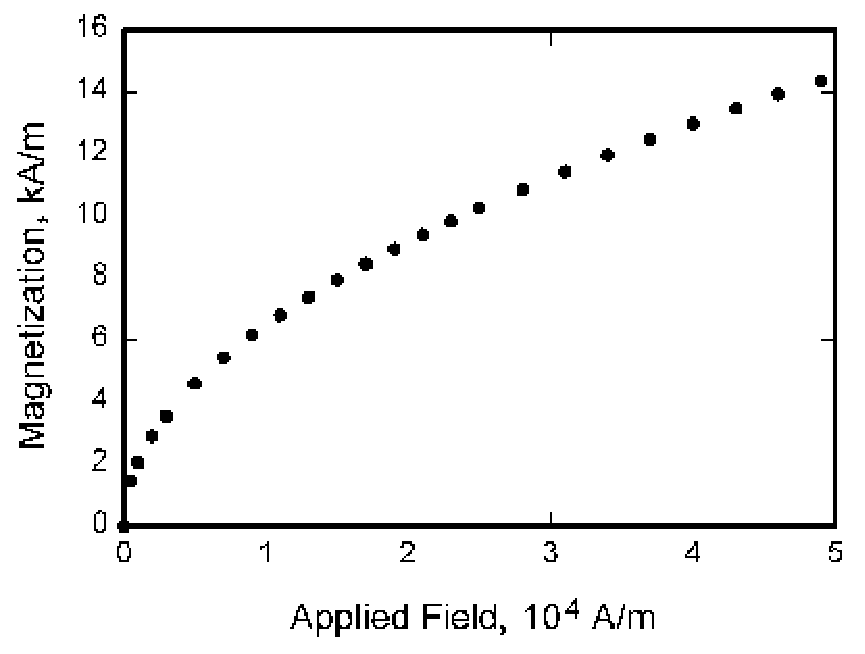
\includegraphics{figure_magnet}
 \caption{Magnetization as a function of applied field, which has
   borders so thick that they overwhelm the data and for some reason the
   ordinate label is rotated 90 degrees to make it difficult to
   read. This figure also demonstrates the dangers of using a bitmap
   as opposed to a vector image.}
 \label{f:magnetic_field}
\end{wrapfigure}

Place figure captions below all figures; place table titles above the
tables.%
\footnote{Please do not include captions as part of the figure image
itself.}
If your figure has multiple parts, include the labels ``a),'' ``b),''
and so on, below each subfigure and above the figure caption.
This can be accomplished with the \pkg{subfigure} package.
Please verify that the figures and tables you mention in the text
actually exist by using \LaTeX's \verb|\label| and \verb|\ref| mechanisms
and verifying that there are no undefined references during typesetting.

When citing a figure in the text, use ``figure'' as ``Fig., often used
to refer to graphics, is an ugly abbreviation and is not worth the two
spaces saved.''\cite{tufte:83bk}
Do not abbreviate ``table'' either.
Each different type of illustration (i.e., figures, tables, or
images) should be numbered sequentially with relation to other
illustrations of the same type.

Figure axis labels are often a source of confusion.
Use words rather than symbols.
As in the example to the right, write the quantity ``Magnetization''
rather than just ``M.''
Do not enclose units in parenthesis, but rather separate them from the
preceding text by commas.
Do not label axes only with units.
As in figure~\ref{f:magnetic_field}, for example, write ``Magnetization,
A/m'' or ``Magnetization, A m-1,'' not just ``A/m.''
Do not label axes with a ratio of quantities and units.
For example, write ``Temperature, K,'' not ``Temperature/K.''

Multipliers can be especially confusing.
Write ``Magnetization, kA/m'' or ``Magnetization, 103 A/m.''
Do not write ``Magnetization (A/m) $\times$ 1000'' because the reader
would not then know whether the top axis label in
figure~\ref{f:magnetic_field} meant 16000~A/m or 0.016~A/m.
Figure labels must be legible, approximately 8--12 point type.
Use of the \pkg{psfrag} package can facilitate this, but it makes
generating a PDF version of your paper difficult.

Figures and tables are referred to as `Floats' in \LaTeX, reflecting
their floating nature.
They are typically numbered whether or not they have a caption and they
are floated to the first available position near the first reference to
that figure/table within the text.
This is accomplished by placing the figure/table environment after
their first reference.
The environment can even be placed mid-sentence as long as \LaTeX's
comment character, \%, is used properly to prevent a paragraph break or
extra spaces.
By default, floats are placed at the top of the first available page,
the bottom of the page, or one a page consisting entirely of floats.

An example of coding a standard \verb|{figure}| is given below:
\begin{Verbatim}
 \begin{figure}
   \includegraphics{magetic_field}
   \caption{Magnetization as a function of applied field, which has
     borders so thick that they overwhelm from the data.}
   \label{f:magnetic_field}
 \end{figure}
\end{Verbatim}

\begin{table}
 \begin{center}
  \begin{threeparttable}
   \caption{This is an example of a \pkg{threeparttable} which uses the
     \pkg{dcolumn} package to allow for columns to be aligned on decimal
     points.}
   \label{t:threepart}
   \begin{tabular}{lcdd}
    First head\tnote{*}  &
    Second head &
    \multicolumn{1}{c}{Third head} &
    \multicolumn{1}{c}{$V_M(r)$} \\\hline
    center & doctor &  0.2  & 10.55 \\  
    tab    & dentist &  0.15 & 33.12 \\ 
    worse  & man\tnote{\ensuremath{\dagger}} & 10.58 & 45.10 \\ 
    better & home & 43.9  & 12.34 \\
   \end{tabular}
   \begin{tablenotes}
    \item[*] This is a table footnote, which to span multiple lines, has
      been greatly extended in length contrary to reason.
    \item[\ensuremath{\dagger}] A much shorter table footnote.
   \end{tablenotes}
  \end{threeparttable}
 \end{center}
\end{table}
Tables with footnotes, such as table~\ref{t:threepart},
can be coded using the \pkg{threeparttable} package as follows:
\begin{Verbatim}
 \begin{table}
  \begin{center}
   \begin{threeparttable}
    \caption{This is an example of table caption.}
    \label{t:wordtable}
    \begin{tabular}{ccdd}
     First head\tnote{a}  &
     Second head\tnote{b} &
     \multicolumn{1}{c}{Third head} &
     \multicolumn{1}{c}{$V_M(r)$} \\\hline
     Left & Word entries &  0.2  & 10.55 \\  
     Left & Word entries &  0.15 & 33.12 \\ 
     Left & Word entries & 10.58 & 45.10 \\ 
     Left & Word entries & 43.9  & 12.34 \\
    \end{tabular}
    \begin{tablenotes}
     \item[a] This is a table footnote, which to span multiple lines, has
              been greatly extended in length contrary to reason.
     \item[b] A much shorter table footnote.
    \end{tablenotes}
   \end{threeparttable}
  \end{center}
 \end{table}
\end{Verbatim}

\subsection{Equations, Numbers, Symbols, and Abbreviations}

Equations are centered and numbered consecutively, with equation
numbers in parentheses flush right, as in Eq.~\ref{e:function}.
\begin{equation}
 \label{e:function}
 \int_{0}^{r_{2}} F(r,\varphi)\,dr\,d\varphi =
    \left[ \sigma r_{2}/(2\mu_{0}) \right] \cdot
    \int_{0}^{\infty} \exp(-\rho|z_{j}-z_{i}|) \lambda^{-1} 
\end{equation}
Equation~\ref{e:function} is coded as below:
\begin{Verbatim}
 \begin{equation}
  \label{e:function}
  \int_{0}^{r_{2}} F(r,\varphi)\,dr\,d\varphi =
     \left[ \sigma r_{2}/(2\mu_{0}) \right] \cdot
     \int_{0}^{\infty} \exp(-\rho|z_{j}-z_{i}|) \lambda^{-1}
 \end{equation}
\end{Verbatim}
A sample equation is included below, formatted using the preceding
instructions.
To make your equation more compact, you can use the solidus ($/$), the
exp function, or appropriate exponents.
Use parentheses to avoid ambiguities in denominators.
\begin{equation}
  \label{e:displace}
  \mathbf{J}_i\cdot\Delta\underline{x}_{i+1}=-\underline{f}_i
\end{equation}
\nomenclature{$J$}{Jacobian Matrix}
\nomenclature[b$i$]{$i$}{Variable number}
\nomenclature[g$\Delta$]{$\Delta x$}{Variable displacement vector}
\nomenclature{$f$}{Residual value vector}
\nomenclature{$x$}{Variable value vector}
\begin{equation}
  \label{e:newton}
  F=m\alpha
\end{equation}
\nomenclature{$F$}{Force, N}
\nomenclature{$m$}{Mass, kg}
\nomenclature[g$\alpha$]{$\alpha$}{Acceleration, m/s\textsuperscript{2}}

The \verb|fleqnarray| environment is used to display a sequence of
equations or inequalities. It is very much like a three-column
\verb|array| environment, with consecutive rows separated by
\verb|\\| and consecutive items within a row separated by an \&.
\begin{eqnarray}
&&\sum_{i\in H} p^0\cdot w^{0i}=\sum_i M^i (p^0) =
  \sum_i\left[p^0\cdot r^i + \sum_j \alpha^{ij} (p^0\cdot
  y^{0j})\right]\nonumber\\
&&{\qquad}= p^0 \cdot \sum_i r^i + p^0 \cdot \sum_i
\sum_i \alpha^{ij}
\end{eqnarray}
An equation number is placed on every line unless that line has a
\verb|\nonumber| command.

Be sure that the symbols in your equation are defined before the
equation appears, or immediately following.
In this case the \pkg{nomencl} package is used to automatically generate
the nomenclature section.

Italicize symbols ($T$ might refer to temperature, but T is the unit
Tesla).
Refer to ``Eq. (1),'' not ``(1)'' or ``equation (1)'' except at the
beginning of a sentence: ``Equation (1) is phat.''
Equations can be labeled other than ``Eq.'' should they represent
inequalities, matrices, or boundary conditions.
If what is represented is really more than one equation, the
abbreviation ``Eqs.'' can be used.

Define abbreviations and acronyms the first time they are used in the
text, even after they have already been defined in the abstract.
Very common abbreviations such as AIAA, SI, ac, and dc do not have to be
defined.
Abbreviations that incorporate periods should not have spaces: write
``P.R.,'' not ``P. R.''
Delete periods between initials if the abbreviation has three or more
initials; e.g., U.N. but ESA.\@
Do not use abbreviations in the title unless they are unavoidable (for
instance, ``AIAA'' in the title of this article).

\subsection{General Grammar and Preferred Usage}

Use only one space after periods or colons. Hyphenate complex
modifiers: ``zero-field-cooled magnetization.''
Avoid dangling participles, such as, ``Using Eq. (1), the potential was
calculated.''
[It is not clear who or what used Eq. (1).]
Write instead ``The potential was calculated using Eq. (1),'' or ``Using
Eq. (1), we calculated the potential.''

Use a zero before decimal points: ``0.25,'' not ``.25.''
Use ``cm$^3$,'' not ``cc.''
Indicate sample dimensions as ``0.1 cm $\times$ 0.2 cm,'' not ``0.1
$\times$ 0.2~cm$^2$.''
The preferred abbreviation for ``seconds'' is ``s,'' not ``sec.''
Do not mix complete spellings and abbreviations of units: use
``Wb/m$^2$'' or ``webers per square meter,'' not ``webers/m$^2$.''
When expressing a range of values, write ``7 to 9'' or ``7--9,'' not
``7~9.''

A parenthetical statement at the end of a sentence is punctuated
outside of the closing parenthesis (like this).
(A parenthetical sentence is punctuated within parenthesis.)
In American English, periods and commas are placed within quotation
marks, like ``this period.''
Other punctuation is ``outside''! Avoid contractions; for example, write
``do not'' instead of ``don't.''
The serial comma is preferred: ``A, B, and C'' instead of ``A, B and C.''

If you wish, you may write in the first person singular or plural and
use the active voice (``I observed that\ldots'' or ``We observed that\ldots''
instead of ``It was observed that�'').
Remember to check spelling.
If your native language is not English, please ask a native
English-speaking colleague to proofread your paper.

The word ``data'' is plural, not singular (i.e., ``data are,'' not ``data
is'').
The subscript for the permeability of vacuum $\mu_0$ is zero, not a
lowercase letter ``oo.''
The term for residual magnetization is ``remanence''; the adjective is
``remanent''; do not write ``remnance'' or ``remnant.''
The word ``micrometer'' is preferred over ``micron'' when spelling out
this unit of measure.
A graph within a graph is an ``inset,'' not an ``insert.''
The word ``alternatively'' is preferred to the word ``alternately''
(unless you really mean something that alternates).
Use the word ``whereas'' instead of ``while'' (unless you are referring
to simultaneous events).
Do not use the word ``essentially'' to mean ``approximately'' or
``effectively.''
Do not use the word ``issue'' as a euphemism for ``problem.''
When compositions are not specified, separate chemical symbols by
en-dashes; for example, ``NiMn'' indicates the intermetallic compound
Ni$_{0.5}$Mn$_{0.5}$ whereas ``Ni--Mn'' indicates an alloy of some
composition Ni$_{x}$Mn$_{1-x}$.

Be aware of the different meanings of the homophones ``affect'' (usually
a verb) and ``effect'' (usually a noun), ``complement'' and
``compliment,'' ``discreet'' and ``discrete,'' ``principal'' (e.g.,
``principal investigator'') and ``principle'' (e.g., ``principle of
measurement''). Do not confuse ``imply'' and ``infer.''

Prefixes such as ``non,'' ``sub,'' ``micro,'' ``multi,'' and ``ultra''
are not independent words; they should be joined to the words they
modify, usually without a hyphen.
There is no period after the ``et'' in the abbreviation ``et al.''
The abbreviation ``i.e.,'' means ``that is,'' and the abbreviation
``e.g.,'' means ``for example'' (these abbreviations are not
italicized).
An excellent source of more detailed style and formatting instructions
can be found in the AIAA style guide, {\it AIAA Style} (available from AIAA
upon request).

\section{Conclusion}

A conclusion section is not required, though it is preferred.
Although a conclusion may review the main points of the paper, do not
replicate the abstract as the conclusion.
A conclusion might elaborate on the importance of the work or suggest
applications and extensions.%
\footnote{The conclusion section is the last section of
  the paper that should be numbered.
  The appendix (if present), acknowledgment, and references should be
  listed without numbers.}

\section*{Appendix}

An appendix, if needed, should appear before the acknowledgments.
Use the 'starred' version of the \verb|\section| commands to avoid
section numbering.

\section*{Acknowledgments}

The preferred spelling of the word ``acknowledgment'' in American
English is without the ``e'' after the ``g.''
Avoid expressions such as ``One of us (S.B.A.) would like to thank\ldots[.]''
Instead, write ``F. A. Author thanks\ldots[.]''
Sponsor and financial support acknowledgments are also to be listed in
the acknowledgments section.

% produces the bibliography section when processed by BibTeX
\bibliography{bibtex_database}
\bibliographystyle{aiaa}

\end{document}

% $Id: author_guide.tex,v 1.3 2004/04/03 14:20:25 kleb Exp $

